\chapter{Introduction}\label{ch:Introduction}
As technology progressively becomes more and more advanced the dream of self driving cars continues to shed the fiction of its science-fiction classification. 
In our daily lives, Tesla's semi automatic cars are often seen. This works as a reminder of one autonomy is currently being used commercially in the automotive industry. \\
When describing the concept by its component parts, one of the main features becomes its capability to reliably move from one destination to another. However the capability of doing this is build upon the ability to autonomously sense the surrounding areas and navigating them. \\ To truly implement full autonomy in cars they need to be able to reliably avoid collisions and accident with surrounding obstacles, pedestrians etc.
\\
\color{blue}
\subsection{Project scope}
The design of a car with any degree of autonomy, consists of several dependent and independent systems and subsystems. These systems work together to ensure a safe and reliable user experience. Simplified these systems can be differentiated as seen on the brainstorm figure \ref{fig:AutoCarSysPic}.\\
This project will focus on investigating and developing a system with the focus on the cars ability to perceive the surroundings and interpret it.

\begin{figure}[H]
 \centering
  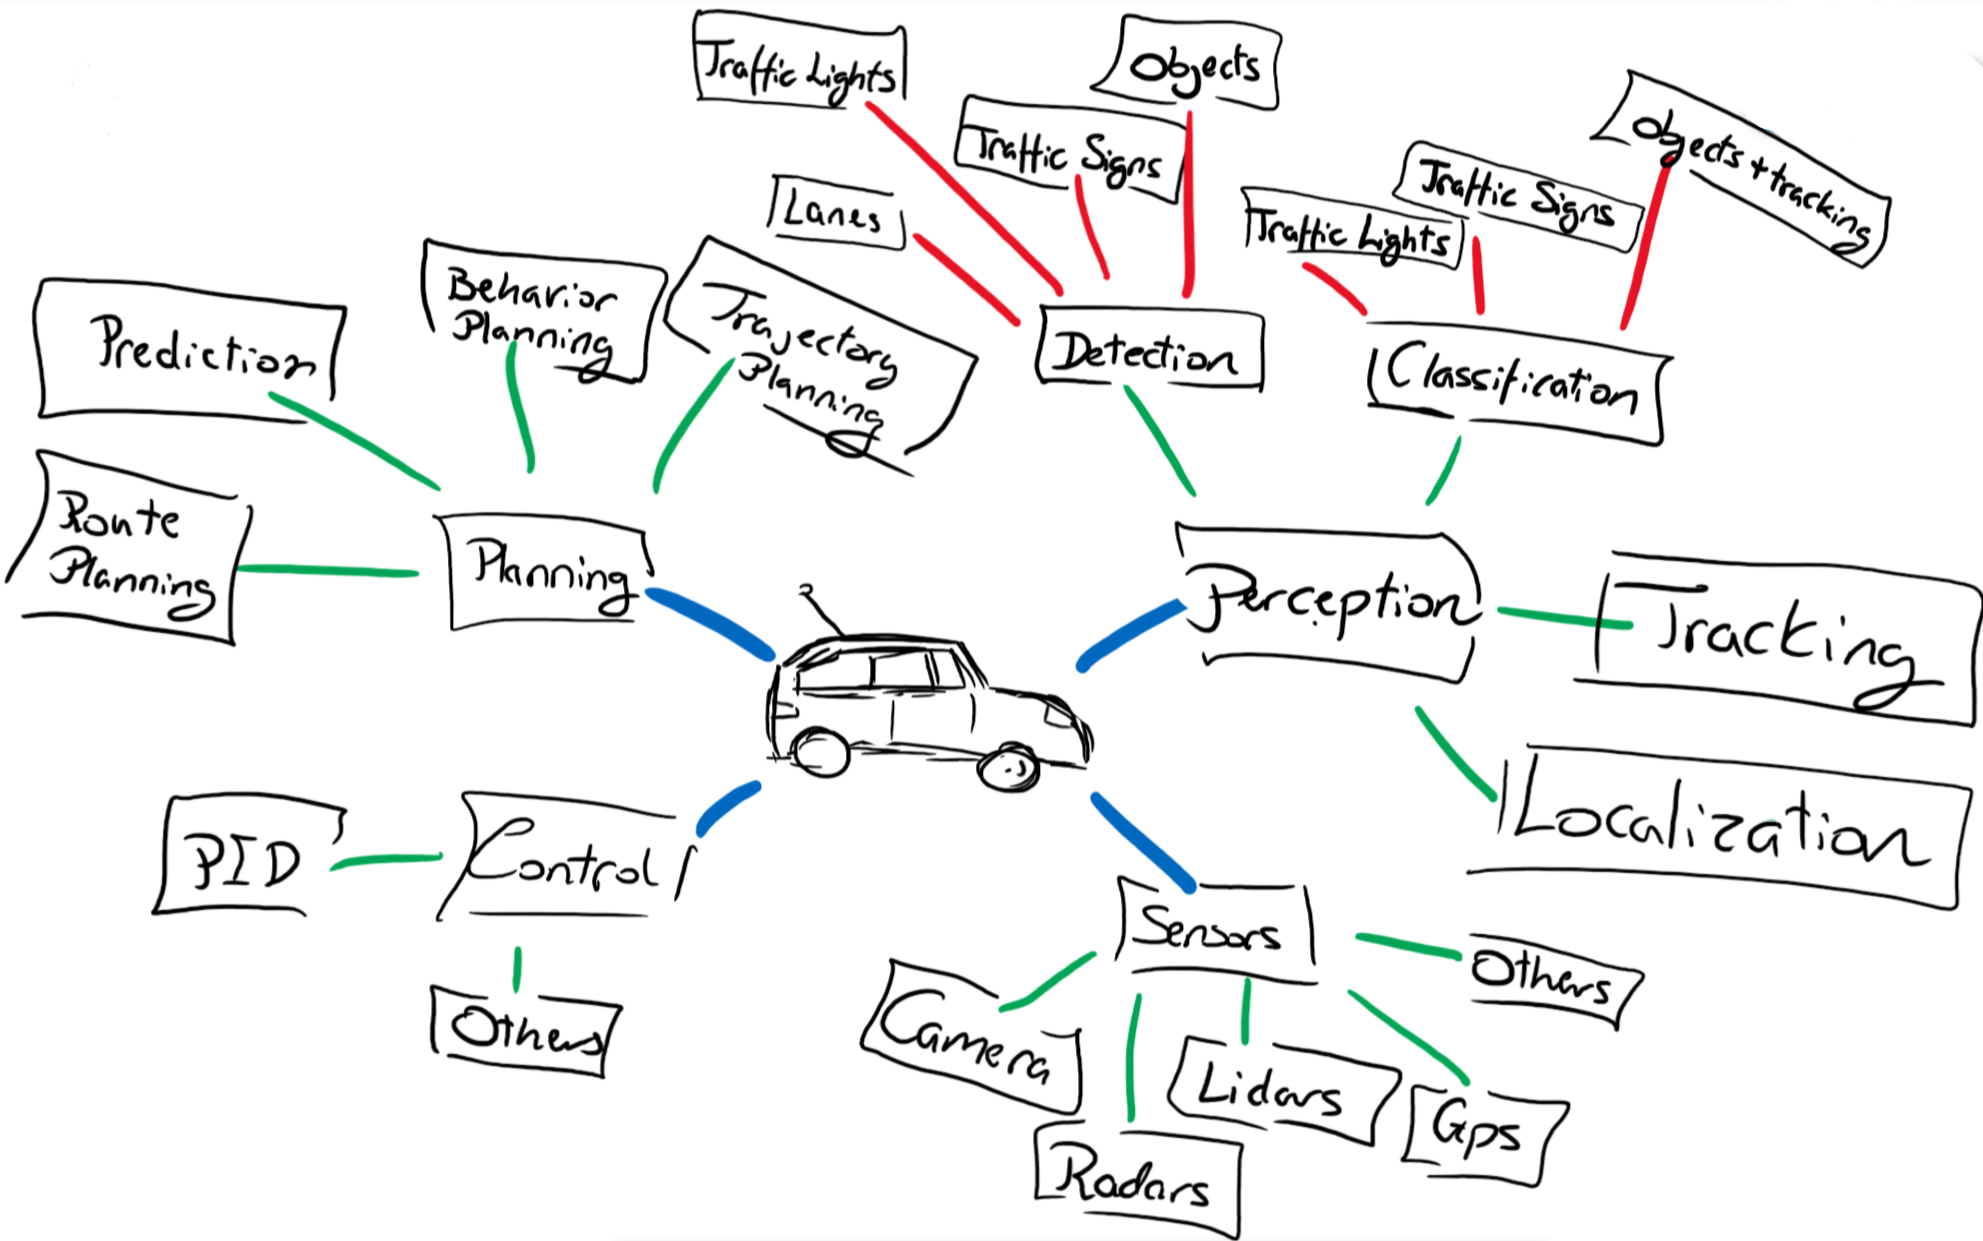
\includegraphics[width=\textwidth]{Figures/ConAnalysis/General/AutoCarSystems2.png}
  \caption{Brainstorm sketch regarding the basic systems and sub-systems of an autonomous car, with supplementing categories  from\cite{AutoCarSys:online}}
  \label{fig:AutoCarSysPic}
\end{figure}

Figure \ref{fig:AutoCarSysPic} shows a brainstorm of the different systems and their subsystems required for an autonomous car to work. It consists of four main branches namely the \textit{"planning, control, perception and} \textit{sensor"} branches. \\
Each of these four branches has several subsystems. Eg. the perception branch consists of both a detecting and a classifying subsystem. The detection subsystem would be responsible for using the sensor data to detect obstacles and the local environment while the classification subsystem would classify the detected objects into preset classes, eg. \textit{“moving objects”}, \textit{“traffic lights”}, \textit{“driving lanes”} and \textit{“traffic signs”} among other specific objects relevant for safe driving.

This project has the goal of developing a proof of concept of a perception subsystem (the "perception branch" on the figure \ref{fig:AutoCarSysPic}) of an autonomous car. As such the focus of the contextual analysis will be in the "perception" subsystem and to a degree "sensors" in order to determine what data would be relevant for the perception system to use. \\

A perception system would need to perceive the surrounding area and map regardless of weather conditions. \\
It should be able to identify the road in the created map and follow it while avoiding and classifying any possible obstacles, be they moving or stationary. 


\section{Initial Problem Formulation}
The initial problem formulation will serve as a framework to guide the focus of the problem analysis towards a delimitation and requirements list.\\ \todo[inline]{Might need a revisit}

   \textbf{ \textit{How can a perception system for an autonomous cars, reliably detect and classify their surroundings as to avoid both stationary and moving obstacles.}}\\

%To answer this the problem analysis will be focusing on:
%\todo[inline]{Reformulate the questions to an outline}
%\begin{enumerate}
%\item  What sensors would be best suited for sensing the surroundings and %identifying obstacles.
%\item  What legal requirements would affect such a system.
%\item Are there any existing solutions.
%\item   How can objects be identified from sensor data.
%\item  How to differentiate between moving  and stationary obstacles.
%\item  How can the movements of live obstacles be predicted.
%\end{enumerate}

\subsection{Outline}
In the following problem analysis there will be looked into the different technologies already existing regarding autonomous driving, as well as some definitions between different levels of autonomy. Afterwards the safety will be investigated in a risk assessment and with respect to the legislation in Denmark. Furthermore a discussion concerning the ethics of autonomous vehicles will look into who is responsible in case of a crash and how different ways to avoid a crash might be ethically wrong since somebody else might be harmed. Next, different sensors will be evaluated with focus on their advantages and disadvantages. The problem analysis will end up in a conclusion which leads into the requirements and delimitations for the solution of the project. With that a final problem formulation is formed.
\color{black}